\chapter{Proposed Work}
\label{chap:proposed_work}
\label{chap:proposed_framework}
\label{chap:system_model}

The literature survey in Chapter~\ref{chap:literature_review} identified two fundamental open challenges in edge-based network intrusion detection: first, how a resource-constrained gateway operating under a closed-world assumption can autonomously detect that incoming traffic represents a previously unseen zero-day attack; and second, how the local detection model can rapidly incorporate the novel threat on-device without inducing catastrophic forgetting of previously learned traffic classes or exceeding edge hardware boundaries.

This chapter details the design, theoretical motivation, mathematical formulation, and system architecture of the proposed two-stage continual intrusion detection framework. Section~\ref{sec:algorithm_design} establishes the formal design requirements, details each functional module of the architecture, provides the mathematical derivation of the Isolation Forest anomaly scoring mechanism, analyzes tree-splitting dynamics and Gini impurity under class imbalance, and formulates the volume-aware Dynamic Replay rule. Section~\ref{sec:datasets_platform} describes the TON\_IoT network benchmark corpus, the feature preprocessing and de-identification protocol, the leave-one-attack-out evaluation methodology, and the software and hardware execution platform.

\section{Algorithm Design}
\label{sec:algorithm_design}

The proposed framework executes directly on an IoT edge gateway, operating across two coordinated stages: an inline line-rate detection and screening stage (Stage~1), and an on-demand on-device adaptation stage (Stage~2). In Stage~1, every incoming bidirectional network flow is classified by an optimized supervised Random Forest classifier~\cite{breiman2001random} and simultaneously scored by an unsupervised Isolation Forest novelty screener~\cite{liu2008isolation}. The Random Forest assigns known flow categories with high throughput, while the Isolation Forest evaluates isolation depth to identify anomalous traffic distributions that deviate from known training baselines.

In Stage~2, which executes only upon verification of a novel attack by security personnel, the gateway dynamically calculates a proportional historical replay quota, samples a balanced exemplar buffer from local memory, and retrains the classifier on the merged dataset in under 0.1~seconds. Figure~\ref{fig:proposed_architecture} illustrates the functional interaction and dataflow across all seven system modules.

\begin{figure}[htpb]
  \centering
  \tikzstyle{block} = [rectangle, line width=0.75pt, draw, text centered, minimum height=10mm, text width=34mm]
  \tikzstyle{line} = [draw, line width=0.75pt, -latex']
  \begin{tikzpicture}
    \node [block] (flows)   at (0, 0)      {\bf\footnotesize Incoming IoT Flows $\mathbf{x} \in \mathbb{R}^d$};
    \node [block] (prep)    at (0, -1.6)   {\bf\footnotesize M1: Flow Preprocessing};
    \node [block] (rf)      at (-3.4, -3.2){\bf\footnotesize M2: Random Forest Classifier};
    \node [block] (iso)     at (3.4, -3.2) {\bf\footnotesize M3: Isolation Forest Screener};
    \node [block] (label)   at (-3.4, -5.0){\bf\footnotesize Predicted Label to Operator};
    \node [block] (analyst) at (3.4, -5.0) {\bf\footnotesize M4: Analyst Verification ($\mathcal{D}_{\text{new}}$, $M$ flows)};
    \node [block] (buffer)  at (3.4, -6.8) {\bf\footnotesize M5: Dynamic Replay Buffer Manager};
    \node [block] (adapt)   at (-3.4, -6.8){\bf\footnotesize M6: Adaptation Engine};
    \node [block] (eval)    at (-3.4, -8.5){\bf\footnotesize M7: Evaluation Module};
    % Draw edges
    \path [line] (flows) -- (prep);
    \path [line] (prep) -- (rf);
    \path [line] (prep) -- (iso);
    \path [line] (rf) -- (label);
    \path [line] (iso) -- node[right] {\footnotesize alert} (analyst);
    \path [line] (analyst) -- (buffer);
    \path [line] (buffer) -- node[above] {\footnotesize $\mathcal{B} \cup \mathcal{D}_{\text{new}}$} (adapt);
    \path [line] (adapt.west) -- (-5.5, -6.8) -- (-5.5, -3.2) -- (rf.west);
    \node at (-6.4, -5.0) {\footnotesize updated};
    \node at (-6.4, -5.35) {\footnotesize model};
    \path [line] (adapt) -- (eval);
  \end{tikzpicture}
  \caption{Architectural overview of the proposed two-stage continual intrusion detection framework showing operational modules M1 through M7}
  \label{fig:proposed_architecture}
\end{figure}

\subsection{Design Requirements}
\label{subsec:requirements}

The operational requirements of the system are dictated by the physical and architectural constraints of IoT edge computing. In a typical deployment, heterogeneous field devices (such as smart sensors, industrial programmable logic controllers, security cameras, and environmental monitors) route communication through an edge gateway appliance. The gateway is situated at the boundary between the local IoT subnet and external cloud or corporate networks. While the gateway is the sole device capable of observing aggregate bidirectional traffic, it possesses constrained computational and storage resources. Transmitting complete raw packet captures to a remote cloud data center for retraining is frequently infeasible due to wide-area bandwidth costs, high latency, and privacy regulations governing industrial telemetry.

\subsubsection{Functional requirements}
The architecture must satisfy four primary functional requirements:
\begin{enumerate}
    \item[\textbf{R1.}] \textbf{High-Accuracy Classification of Familiar Traffic:} The gateway must inspect network flows at line rate and assign them to known benign or threat categories with multi-class classification accuracy, precision, and recall comparable to conventional centralized supervised intrusion detectors.
    \item[\textbf{R2.}] \textbf{Autonomous Unsupervised Anomaly Flagging:} Because a supervised classifier is mathematically incapable of predicting a class label absent from its training taxonomy, an independent, unsupervised scoring mechanism must monitor traffic in parallel to flag unfamiliar, out-of-distribution flows without requiring prior attack signatures or labels.
    \item[\textbf{R3.}] \textbf{Rapid Integration of Confirmed Novel Threats:} Upon confirmation of an ongoing zero-day incident by an operator or security analyst, who provides a small verified batch $\mathcal{D}_{\text{new}}$ of $M$ flows, the framework must expand its classification taxonomy from $K$ to $K+1$ classes, achieving high macro and per-class F1 performance on subsequent instances of the new attack.
    \item[\textbf{R4.}] \textbf{Strict Retention of Historical Knowledge:} Integrating the novel class must not compromise previously acquired classification boundaries. Both the average forgetting metric ($\mathcal{F}_{\text{avg}}$) and the worst-case single-class forgetting metric ($\mathcal{F}_{\max}$) across the original $K$ classes must remain tightly bounded.
\end{enumerate}

\subsubsection{Non-functional requirements}
The practical feasibility of edge deployment imposes three critical non-functional constraints:
\begin{enumerate}
    \item[\textbf{R5.}] \textbf{Strict Memory and Storage Bounds:} The total volume of historical telemetry retained for model adaptation must remain constrained under a strict ceiling ($\le 5{,}000$ flows, corresponding to less than 1~MB of RAM), preventing exhaustion of flash memory and local volatile buffers.
    \item[\textbf{R6.}] \textbf{Sub-Second On-Device Adaptation Latency:} Model retraining must execute on general-purpose gateway processor cores within a fraction of a second ($\le 0.1$~s), ensuring that updated decision boundaries are deployed immediately without stalling line-rate flow inspection.
    \item[\textbf{R7.}] \textbf{Robust Invariance to Attack Volume:} The framework must satisfy R3 through R6 regardless of whether the emerging attack manifests as a stealthy, low-volume trickle (e.g., hundreds of flows) or a massive volumetric flood (e.g., tens of thousands of flows).
\end{enumerate}

\subsubsection{Operational Assumptions}
The framework operates under standard edge computing trust assumptions:
\begin{itemize}
    \item The gateway hardware platform, operating system kernel, packet capture interface, and local memory buffers are assumed secure against physical compromise and unauthorized tampering.
    \item The framework inspects bidirectional flow-level statistical summaries (such as packet counts, byte volumes, inter-arrival times, and protocol state flags) rather than decrypting deep packet payloads, preserving operational throughput and end-to-end payload encryption.
    \item Ground-truth class labels for novel attack flows are verified by security analysts or upstream automated threat intelligence feeds prior to adaptation; the framework governs how the model learns from these labels on-device.
\end{itemize}

Requirement~R7 represents the core limitation of existing continual learning methods. In real-world IoT networks, different cyber attack families display drastic volumetric divergence. Stealthy reconnaissance and Man-in-the-Middle (MITM) attacks produce sparse, intermittent traffic; in the TON\_IoT benchmark, MITM represents only 0.5\% of the total flow volume. Conversely, denial-of-service floods, ransomware sweeps, and automated cross-site scripting (XSS) scanners generate thousands of flows in rapid succession. A static replay buffer cannot accommodate this dynamic range, necessitating a volume-aware allocation strategy.

\subsection{System Modules}
\label{subsec:modules}

The architecture is partitioned into seven discrete modules (M1 through M7), ensuring modular maintainability and decoupled execution across edge resources.

\subsubsection{M1: Flow preprocessing}
\label{subsubsec:m1_flow_preprocessing}
Module~M1 converts raw bidirectional network flows captured by packet capture engines (e.g., Zeek) into clean, standardized numeric feature vectors $\mathbf{x} \in \mathbb{R}^d$. The preprocessing pipeline applies five deterministic transformation steps:
\begin{enumerate}
    \item \textbf{Missing Value Harmonization:} Dash characters (``--'') and null placeholders common in Zeek logs are mapped to explicit null indicators.
    \item \textbf{De-identification and Bias Prevention:} Network layer source and destination IP addresses, MAC addresses, port numbers, and capture timestamps are stripped. This prevents the supervised models from memorizing specific host addresses or network topologies present in the evaluation testbed.
    \item \textbf{High-Sparsity Feature Pruning:} Telemetry columns exhibiting greater than 50\% missingness across historical baseline traffic are pruned from the feature space.
    \item \textbf{Imputation:} Remaining missing values in numeric continuous features are imputed using the training set median, while categorical attributes are imputed using the training mode.
    \item \textbf{Categorical Encoding:} Categorical attributes, including transport protocols (e.g., TCP, UDP, ICMP) and connection states, are transformed using one-hot encoding. Any novel categorical value observed at test time that was unobserved during initial training is mapped to an all-zero vector.
\end{enumerate}
Crucially, all statistical parameters (imputation medians, modes, and categorical vocabularies) are calculated strictly on the training partition and applied without modification to test streams, preventing data leakage.

\subsubsection{M2: Random Forest classifier}
\label{subsubsec:m2_rf_classifier}
The primary inline inspection engine is a supervised Random Forest ensemble~\cite{breiman2001random} comprising $B = 100$ unpruned decision trees with a maximum depth constraint of 20 levels. Let the historical training dataset be denoted as $\mathcal{D}_{\text{train}} = \{(\mathbf{x}_i, y_i)\}_{i=1}^{N}$, where $\mathbf{x}_i \in \mathbb{R}^d$ and $y_i \in \mathcal{C} = \{1, 2, \dots, K\}$ represents one of $K$ known historical traffic categories.

For an incoming flow vector $\mathbf{x}$, each individual decision tree $b \in \{1, \dots, B\}$ traverses its internal nodes based on orthogonal feature threshold tests until a leaf node is reached. The ensemble aggregates the leaf posterior class probabilities and outputs the majority predicted class label:
\begin{equation}
f_\theta(\mathbf{x}) = \arg\max_{k \in \mathcal{C}} \; \frac{1}{B} \sum_{b=1}^{B} P_b(y = k \mid \mathbf{x}),
\label{eq:rf_prediction}
\end{equation}
where $P_b(y = k \mid \mathbf{x})$ denotes the empirical training class frequency within the leaf node reached by sample $\mathbf{x}$ in tree $b$. 

Decision tree ensembles provide substantial operational advantages for IoT gateway deployment: they natively accommodate mixed-scale tabular features, exhibit scale invariance, require negligible parameter tuning, and execute inference in sub-millisecond timeframes using standard integer and floating-point comparisons on basic CPUs. However, their fundamental structural limitation is that the output space is strictly bounded by the historical label set $\mathcal{C}$. When presented with an emergent zero-day attack vector $\mathbf{x}^* \sim \mathcal{P}_{K+1}$, the ensemble deterministically assigns $\mathbf{x}^*$ to whichever historical class leaf shares the closest proximity in feature space, resulting in silent intrusion evasion.

\subsubsection{M3: Isolation Forest novelty screener}
\label{subsubsec:m3_isolation_screener}
To provide the autonomous anomaly signal mandated by Requirement~R2, Module~M3 operates in parallel with the supervised classifier, evaluating an unsupervised Isolation Forest~\cite{liu2008isolation} consisting of 100 isolation trees.

The Isolation Forest isolates anomalies by exploiting two structural properties of novel attacks: they represent minority instances, and their feature distributions differ significantly from normal baseline traffic. Each isolation tree is constructed by recursively partitioning a randomly sampled subset of training data ($\psi = 256$ samples) along randomly selected feature dimensions $j \in \{1, \dots, d\}$ at split points $\tau \in (\min(x_j), \max(x_j))$ until either all samples are isolated or the tree reaches its maximum depth limit $\lceil \log_2(\psi) \rceil$.

Because anomalous flows occupy sparse regions of the feature space, they require substantially fewer recursive splits to be isolated compared to dense, clustered normal flows. For a flow $\mathbf{x}$, let $h_t(\mathbf{x})$ denote the path length (number of edges traversed) in isolation tree $t$. The anomaly score $s(\mathbf{x}, n)$ over an ensemble of $T$ trees is defined as:
\begin{equation}
s(\mathbf{x}, n) = 2^{-\,\frac{\mathbb{E}[h(\mathbf{x})]}{c(n)}},
\label{eq:isolation_score}
\end{equation}
where $\mathbb{E}[h(\mathbf{x})] = \frac{1}{T}\sum_{t=1}^{T} h_t(\mathbf{x})$ is the average observed path length across all trees, and $c(n)$ is the average path length of unsuccessful searches in a binary search tree constructed over $n$ instances:
\begin{equation}
c(n) = 2 \ln(n - 1) + 2\gamma - \frac{2(n - 1)}{n},
\label{eq:bst_average_depth}
\end{equation}
with $\gamma \approx 0.5772156649$ representing Euler's constant.

The anomaly score exhibits three distinct asymptotic behaviors:
\begin{itemize}
    \item When $\mathbb{E}[h(\mathbf{x})] \to 0$, the anomaly score $s(\mathbf{x}, n) \to 1$, indicating that the instance isolates near the root and represents a high-confidence structural anomaly.
    \item When $\mathbb{E}[h(\mathbf{x})] \to c(n)$, the anomaly score $s(\mathbf{x}, n) \to 0.5$, indicating that the flow exhibits average cluster depth typical of background traffic.
    \item When $\mathbb{E}[h(\mathbf{x})] \to n - 1$, the anomaly score $s(\mathbf{x}, n) \to 0$, indicating that the instance is deeply embedded in dense feature clusters.
\end{itemize}

Module~M3 is fitted exclusively on the baseline training partition using scikit-learn's automatic contamination threshold. It was intentionally left untuned to establish an uncalibrated, generalized screening baseline. Its primary objective is to raise an operational anomaly alert when flow path lengths compress, triggering operator investigation.

\subsubsection{M4: Analyst verification}
\label{subsubsec:m4_analyst_verification}
When the Isolation Forest raises sustained anomaly alerts exceeding baseline thresholds, the suspect flow sequence is routed to an isolated quarantine buffer for verification. An analyst or an external threat intelligence engine reviews the flagged traffic, determines whether the activity represents network equipment misconfiguration or an active cyber attack, and provides confirmed ground-truth labels. 

Upon confirmation, the analyst supplies a batch $\mathcal{D}_{\text{new}} = \{(\mathbf{x}_i, y_i)\}_{i=1}^{M}$ containing $M$ labeled flow instances of the new attack class $y_i = K+1$. In our empirical evaluation protocol, this verification stage is simulated by releasing a 20\% slice of the held-out attack family from the TON\_IoT benchmark.

\subsubsection{M5: Dynamic Replay buffer manager}
\label{subsubsec:m5_dynamic_replay}
Module~M5 governs the composition and sizing of the historical replay buffer, constituting the core algorithmic contribution of this thesis. To understand why conventional continual learning techniques fail on edge tree ensembles, we examine the mathematical mechanics of tree induction under class imbalance.

Unlike deep neural networks that update continuous weight vectors via stochastic gradient descent and can be regularized using weight consolidation~\cite{kirkpatrick2017overcoming}, a Random Forest possesses no static parameters to preserve. A decision tree is induced recursively from the discrete data samples provided to it. At each internal node $s$, the splitting algorithm evaluates candidate feature indices $j$ and split thresholds $\tau$ to maximize the reduction in Gini impurity:
\begin{equation}
\Delta I(s, j, \tau) = I(s) - \frac{|s_L|}{|s|} I(s_L) - \frac{|s_R|}{|s|} I(s_R),
\label{eq:gini_reduction}
\end{equation}
where $s_L = \{\mathbf{x} \in s \mid x_j \le \tau\}$ and $s_R = \{\mathbf{x} \in s \mid x_j > \tau\}$ denote the left and right child subsets, and the node Gini impurity $I(s)$ is given by:
\begin{equation}
I(s) = 1 - \sum_{k=1}^{K+1} p_k^2(s), \qquad p_k(s) = \frac{1}{|s|} \sum_{\mathbf{x}_i \in s} \mathbb{I}(y_i = k).
\label{eq:gini_impurity}
\end{equation}

Notice that in Equation~\eqref{eq:gini_reduction}, the impurity reduction is weighted by the relative sample proportions $\frac{|s_L|}{|s|}$ and $\frac{|s_R|}{|s|}$. Consequently, the candidate splits that isolate the majority class yield the largest numerical reductions in global impurity. When classes are heavily imbalanced, decision trees prioritize early, high-level splits to separate the dominant class, while minority classes are relegated to deep leaf nodes or absorbed into majority leaves due to tree depth constraints.

When updating a model with a new attack $\mathcal{D}_{\text{new}}$ of size $M$, three potential data allocation paradigms exist:
\begin{enumerate}
    \item \textbf{New-Data-Only Adaptation:} Retraining exclusively on $\mathcal{D}_{\text{new}}$ yields a root node where $p_{K+1} = 1$. The historical classes vanish completely from the tree structures, resulting in complete catastrophic forgetting ($F1_{\text{known}} = 0.000$).
    \item \textbf{Full Historical Retraining:} Retraining on the full union $\mathcal{D}_{\text{train}} \cup \mathcal{D}_{\text{new}}$ eliminates forgetting but requires retaining the entire historical archive on the gateway ($N \approx 127{,}787$ flows), violating Requirement~R5. Furthermore, when the novel attack is rare (such as MITM, where $M = 207$), the novel class constitutes less than 0.16\% of the training data. The trees prioritize splitting the dominant known classes, failing to learn the new attack and producing an F1 score of only 0.648.
    \item \textbf{Static Fixed-Size Replay:} Maintaining a static buffer of $k$ samples per known class ($N_{\text{buffer}} = K \cdot k$) bounds memory but creates severe volumetric imbalance when the incoming attack volume $M$ varies.
\end{enumerate}

To quantify this volumetric distortion, we define the \textit{volumetric imbalance ratio} $\rho$:
\begin{equation}
\rho = \frac{M}{K \cdot k}.
\label{eq:volumetric_imbalance_ratio}
\end{equation}
Table~\ref{tab:rho_motivation} illustrates the empirical values of $\rho$ for a fixed buffer of $k = 100$ samples per class ($K = 9$, $N_{\text{buffer}} = 900$ flows) across the four held-out attacks in the TON\_IoT benchmark, alongside the maximum observed forgetting on historical classes.

\begin{table}[!ht]
\centering
\small
\setlength{\tabcolsep}{5pt}
\renewcommand{\arraystretch}{1.2}
\caption{Volumetric imbalance ratio ($\rho$) and maximum observed forgetting ($\mathcal{F}_{\max}$) under a static replay buffer ($k = 100$ flows/class, $K = 9$)}
\label{tab:rho_motivation}
\begin{tabular}{|l|r|r|r|l|}
\hline
\textbf{Held-Out Novel Attack} & \textbf{Batch Size ($M$)} & \textbf{Buffer Size ($K \cdot k$)} & \textbf{Ratio $\rho = \frac{M}{900}$} & \textbf{Max Forgetting ($\mathcal{F}_{\max}$)} \\ \hline
MITM       & 207     & 900 & 0.23 & 0.060 (Negligible) \\
Ransomware & 2{,}853 & 900 & 3.17 & 0.324 (Severe) \\
XSS        & 2{,}903 & 900 & 3.23 & 0.397 (Critical) \\
Backdoor   & 3{,}742 & 900 & 4.16 & 0.279 (Severe) \\ \hline
\end{tabular}
\end{table}

When $\rho \le 1$ (as observed for MITM), the historical buffer preserves adequate representation, keeping maximum forgetting below 0.060. However, when large volumetric attacks arrive ($\rho > 3$), the novel attack flows outnumber each stored historical class by more than 28 to 1. The Gini criterion greedily dedicates tree capacity to partitioning the dominant new attack, causing maximum forgetting to spike drastically up to 0.397.

To neutralize this volumetric distortion, we introduce the **Dynamic Replay Allocation Rule**, which dynamically adjusts the per-class replay quota $k_{\text{dyn}}$ as a function of incoming batch size $M$:
\begin{equation}
k_{\text{dyn}} = \min\!\left( k_{\max},\; \max\!\left( k_{\min},\; \left\lfloor \frac{M}{K} \right\rfloor \right) \right).
\label{eq:dynamic_rule_pw}
\end{equation}

The rule establishes three operational regimes:
\begin{enumerate}
    \item \textbf{Sub-Quota Floor Regime ($M < K \cdot k_{\min}$):} When the new attack batch is small ($M < 900$), the lower bound $k_{\min} = 100$ enforces a baseline presence for every historical class. This floor prevents statistical sample starvation and was empirically determined from buffer sensitivity sweeps (Chapter~\ref{chap:results_and_discussion}).
    \item \textbf{Proportional Scaling Regime ($K \cdot k_{\min} \le M \le K \cdot k_{\max}$):} For moderate to large attacks ($900 \le M \le 5{,}000$), the replay quota expands linearly as $k_{\text{dyn}} = \lfloor M/K \rfloor$. This maintains an equilibrium ratio of $\rho \approx 1.0$, ensuring that the aggregate historical buffer matches the volume of the incoming attack batch.
    \item \textbf{Bounded Hardware Ceiling Regime ($M > K \cdot k_{\max}$):} To guarantee compliance with Requirement~R5, the total buffer size is strictly capped at $N_{\text{cap}} = 5{,}000$ flows, establishing an upper bound of $k_{\max} = \lfloor 5000 / K \rfloor = 555$ flows per class for $K = 9$.
\end{enumerate}

Figure~\ref{fig:dynamic_rule_plot} plots the mathematical trajectory of $k_{\text{dyn}}$ across incoming attack volumes $M$, highlighting the operating points of the four experimental attack scenarios.

\begin{figure}[htpb]
  \centering
  \begin{tikzpicture}
    % axes
    \draw[-latex', line width=0.75pt] (0,0) -- (11.2,0);
    \draw[-latex', line width=0.75pt] (0,0) -- (0,6.2);
    \node at (5.5,-0.75) {\footnotesize New-attack batch size $M$ (flows)};
    \node[rotate=90] at (-1.2,3.0) {\footnotesize Replay quota $k_{\text{dyn}}$ (flows/class)};
    % ticks
    \draw (0,0)   -- (0,-0.12)   node[below] {\scriptsize 0};
    \draw (1.8,0) -- (1.8,-0.12) node[below] {\scriptsize 1000};
    \draw (3.6,0) -- (3.6,-0.12) node[below] {\scriptsize 2000};
    \draw (5.4,0) -- (5.4,-0.12) node[below] {\scriptsize 3000};
    \draw (7.2,0) -- (7.2,-0.12) node[below] {\scriptsize 4000};
    \draw (9.0,0) -- (9.0,-0.12) node[below] {\scriptsize 5000};
    \draw (10.8,0)-- (10.8,-0.12)node[below] {\scriptsize 6000};
    \draw (0,0)   -- (-0.12,0)   node[left] {\scriptsize 0};
    \draw (0,1)   -- (-0.12,1)   node[left] {\scriptsize 100};
    \draw (0,2)   -- (-0.12,2)   node[left] {\scriptsize 200};
    \draw (0,3)   -- (-0.12,3)   node[left] {\scriptsize 300};
    \draw (0,4)   -- (-0.12,4)   node[left] {\scriptsize 400};
    \draw (0,5)   -- (-0.12,5)   node[left] {\scriptsize 500};
    \draw (0,6)   -- (-0.12,6)   node[left] {\scriptsize 600};
    % floor and ceiling
    \draw[dashed] (0,1) -- (10.8,1);
    \node[above] at (9.3,1.02) {\scriptsize floor $k_{\min} = 100$};
    \draw[dashed] (0,5.55) -- (10.8,5.55);
    \node[below] at (9.2,5.50) {\scriptsize ceiling $k_{\max} = 555$};
    % rule
    \draw[line width=1.2pt] (0,1) -- (1.62,1) -- (9.0,5.55) -- (10.8,5.55);
    \node[above] at (3.6,2.5) {\scriptsize $k_{\text{dyn}} = \lfloor M/K \rfloor$};
    % experimental points
    \fill (0.37,1.0)  circle (2pt) node[above right] {\scriptsize MITM (207)};
    \fill (5.14,3.17) circle (2pt) node[above left]  {\scriptsize Ransomware (2{,}853)};
    \fill (5.23,3.22) circle (2pt) node[below right] {\scriptsize XSS (2{,}903)};
    \fill (6.74,4.15) circle (2pt) node[above left]  {\scriptsize Backdoor (3{,}742)};
  \end{tikzpicture}
  \caption{Dynamic Replay quota allocation function ($k_{\text{dyn}}$) versus novel attack batch size ($M$) for $K = 9$ known classes, marking experimental evaluation points}
  \label{fig:dynamic_rule_plot}
\end{figure}

Exemplars for each historical class $c \in \mathcal{C}$ are extracted via uniform random sampling without replacement. If a class contains fewer historical records than $k_{\text{dyn}}$, all available records for that class are included in the buffer.

\subsubsection{M6: Adaptation engine}
\label{subsubsec:m6_adaptation_engine}
Module~M6 merges the dynamically sampled historical buffer $\mathcal{B}$ with the novel attack batch $\mathcal{D}_{\text{new}}$ into a unified adaptation dataset $\mathcal{D}_{\text{adapt}} = \mathcal{B} \cup \mathcal{D}_{\text{new}}$ and retrains the Random Forest ensemble on-device. The step-by-step procedural execution is formalized in Algorithm~1.

\begin{table}[htpb]
\centering
\small
\renewcommand{\arraystretch}{1.35}
\caption{Algorithm 1: Dynamic Replay Adaptation Procedure on the Edge Gateway}
\label{alg:dynamic_replay_pw}
\begin{tabular}{|p{13.5cm}|}
\hline
\textbf{Input:} Historical training corpus $\mathcal{D}_{\text{train}}$, known class label set $\mathcal{C}$ with $K = |\mathcal{C}|$, confirmed novel attack batch $\mathcal{D}_{\text{new}}$ with volume $M = |\mathcal{D}_{\text{new}}|$, per-class lower bound $k_{\min}$, per-class upper bound $k_{\max}$. \\
\textbf{Output:} Retrained, deployed Random Forest model $f_{\theta'}$ predicting over expanded taxonomy $\mathcal{C} \cup \{K+1\}$. \\ \hline
1: Measure confirmed novel attack batch volume $M \leftarrow |\mathcal{D}_{\text{new}}|$ and count known classes $K \leftarrow |\mathcal{C}|$. \\
2: Compute volume-aware per-class quota: $k_{\text{dyn}} \leftarrow \min\!\left(k_{\max}, \max\!\left(k_{\min}, \lfloor M/K \rfloor\right)\right)$. \\
3: Initialize empty replay buffer: $\mathcal{B} \leftarrow \emptyset$. \\
4: \textbf{for each} known class $c \in \mathcal{C}$ \textbf{do} \\
5: \hspace{0.5cm} Filter historical partition: $\mathcal{D}_c \leftarrow \{(\mathbf{x}, y) \in \mathcal{D}_{\text{train}} \mid y = c\}$. \\
6: \hspace{0.5cm} Determine sampling target: $n_c \leftarrow \min(k_{\text{dyn}}, |\mathcal{D}_c|)$. \\
7: \hspace{0.5cm} Draw $n_c$ exemplars uniformly at random: $\mathcal{B}_c \leftarrow \text{UniformSample}(\mathcal{D}_c, n_c)$. \\
8: \hspace{0.5cm} Accumulate into replay buffer: $\mathcal{B} \leftarrow \mathcal{B} \cup \mathcal{B}_c$. \\
9: \textbf{end for} \\
10: Assemble adaptation dataset: $\mathcal{D}_{\text{adapt}} \leftarrow \mathcal{B} \cup \mathcal{D}_{\text{new}}$. \\
11: Induce updated ensemble: $f_{\theta'} \leftarrow \text{TrainRandomForest}(\mathcal{D}_{\text{adapt}})$. \\
12: Atomically deploy $f_{\theta'}$ into the active Stage~1 inspection pipeline. \\ \hline
\end{tabular}
\end{table}

\textbf{Computational Complexity and Execution Latency:} The computational complexity of inducing a Random Forest of $B$ trees on an adaptation set containing $n$ samples with $d$ features is approximately $\mathcal{O}(B \cdot d' \cdot n \log n)$, where $d' = \sqrt{d}$ represents the randomized feature subset evaluated at each node split. 

By replacing the full training repository ($N \approx 127{,}787$ flows) with the bounded adaptation dataset ($n \approx 1{,}107$ to $7{,}477$ flows), the volume of training instances is reduced by 94.1\% to 99.1\%. On standard gateway processors, this reduction decreases training latency from over 0.70~seconds down to between 0.04 and 0.09~seconds.

Figure~\ref{fig:workflow} illustrates the end-to-end operational execution of the framework during live gateway operation. The overwhelming majority of network flows execute exclusively on the fast path (Stage~1), undergoing parallel inference by M2 and M3. Only when anomalous flows trigger sustained M3 alerts does the gateway execute the adaptation loop (M4 through M7), ensuring zero downtime for inline traffic filtering.

\begin{figure}[htpb]
  \centering
  \tikzstyle{block} = [rectangle, draw, line width=0.75pt, text width=54mm, text centered, minimum height=9mm]
  \tikzstyle{line} = [draw, line width=0.75pt, -latex']
  \begin{tikzpicture}
    \node[block] (a) at (0, 0)    {\bf\footnotesize Flow arrives at gateway \& is preprocessed (M1)};
    \node[block] (b) at (0, -1.5) {\bf\footnotesize Classify with RF (M2) \& score with IF (M3)};
    \node[block] (c) at (0, -3.0) {\bf\footnotesize Anomaly alert raised by M3?};
    \node[block] (d) at (0, -4.5) {\bf\footnotesize Analyst confirms new attack $\mathcal{D}_{\text{new}}$? (M4)};
    \node[block] (e) at (0, -6.0) {\bf\footnotesize Compute $k_{\text{dyn}}$ from $M$ \& sample buffer $\mathcal{B}$ (M5)};
    \node[block] (f) at (0, -7.5) {\bf\footnotesize Retrain classifier on $\mathcal{B} \cup \mathcal{D}_{\text{new}}$ (M6)};
    \node[block] (g) at (0, -9.0) {\bf\footnotesize Evaluate metrics \& deploy updated model (M7)};
    \node[block, text width=30mm] (r) at (5.2, -3.0) {\bf\footnotesize Report predicted label};
    \path[line] (a) -- (b);
    \path[line] (b) -- (c);
    \path[line] (c) -- node[right] {\scriptsize yes} (d);
    \path[line] (d) -- node[right] {\scriptsize yes} (e);
    \path[line] (e) -- (f);
    \path[line] (f) -- (g);
    \path[line] (c) -- node[above] {\scriptsize no} (r);
    \path[line] (d.east) -- (5.2, -4.5) -- node[right] {\scriptsize no} (r.south);
    \path[line] (g.west) -- (-3.6, -9.0) -- (-3.6, -1.5) -- (b.west);
    \node at (-4.3, -5.2) {\scriptsize next};
    \node at (-4.3, -5.55) {\scriptsize flows};
  \end{tikzpicture}
  \caption{Operational flowchart of the two-stage continual intrusion detection framework on an IoT edge gateway}
  \label{fig:workflow}
\end{figure}

\subsubsection{M7: Evaluation module}
\label{subsubsec:m7_evaluation_module}
Module~M7 evaluates the updated model against the functional and non-functional requirements:
\begin{enumerate}
    \item \textbf{Novel Attack Acquisition (Plasticity):} Evaluates the F1 score achieved on the held-out test partition of the new attack class ($F1_{\text{new}}$), assessing compliance with Requirement~R3.
    \item \textbf{Historical Knowledge Retention (Stability):} For each known class $c \in \mathcal{C}$, the drop in per-class F1 score is tracked:
    \begin{equation}
    \Delta_c = F1_c^{\text{before}} - F1_c^{\text{after}}.
    \label{eq:delta_c}
    \end{equation}
    The framework reports both the macro-averaged forgetting ($\mathcal{F}_{\text{avg}}$) and the worst-case maximum forgetting ($\mathcal{F}_{\max}$):
    \begin{equation}
    \mathcal{F}_{\text{avg}} = \frac{1}{K} \sum_{c \in \mathcal{C}} \max(0, \Delta_c), \qquad \mathcal{F}_{\max} = \max_{c \in \mathcal{C}} \Delta_c.
    \label{eq:forgetting_metrics}
    \end{equation}
    Tracking $\mathcal{F}_{\max}$ is essential: in multi-class intrusion detection, a low average forgetting score can obscure the complete failure of a single critical baseline class (e.g., normal operational traffic).
    \item \textbf{Resource Consumption:} Tracks the percentage reduction in required historical exemplar storage relative to full retraining:
    \begin{equation}
    \text{Storage Reduction} = \left( 1 - \frac{|\mathcal{B}|}{|\mathcal{D}_{\text{train}}|} \right) \times 100\%,
    \label{eq:storage_reduction}
    \end{equation}
    alongside wall-clock retraining execution time measured in seconds (Requirement~R6).
\end{enumerate}

\section{Datasets for the study and Platform}
\label{sec:datasets_platform}

\subsection{TON\_IoT Network Dataset}
\label{subsec:toniot_dataset}

All experiments are conducted using the network telemetry portion of the contemporary TON\_IoT dataset~\cite{alshammari2020toniot}, collected by the Cyber Range Lab of UNSW Canberra. The TON\_IoT testbed captures realistic telemetry generated across a multi-tier Internet of Things infrastructure, integrating physical sensor nodes (e.g., temperature, humidity, motion, light, and garage door sensors), gateway aggregators, virtual machines, and cloud web services.

The network traffic component was captured in raw packet capture (pcap) files and processed using Zeek into connection summaries. The dataset contains 211{,}043 total flow records characterized by 44 attributes, comprising benign normal operations and nine representative modern cyber attack categories. Table~\ref{tab:class_distribution_pw} details the empirical record counts and class proportions across the dataset.

\begin{table}[!t]
\centering
\small
\setlength{\tabcolsep}{5pt}
\renewcommand{\arraystretch}{1.2}
\caption{Class distribution of the TON\_IoT network dataset used in this research}
\label{tab:class_distribution_pw}
\begin{tabular}{|l|r|r|p{7.2cm}|}
\hline
\textbf{Traffic Class} & \textbf{Flow Records} & \textbf{Share (\%)} & \textbf{Operational Threat Behavior} \\ \hline
Normal      & 50{,}000 & 23.69 & Benign sensor telemetry and supervisory traffic \\
Backdoor    & 20{,}000 & 9.48  & Stealthy remote access and command-and-control beacons \\
DDoS        & 20{,}000 & 9.48  & High-rate distributed volumetric UDP/SYN floods \\
DoS         & 20{,}000 & 9.48  & Local volumetric resource exhaustion attacks \\
Injection   & 20{,}000 & 9.48  & Malicious database query and shell command injection \\
Password    & 20{,}000 & 9.48  & High-frequency brute-force dictionary authentication \\
Ransomware  & 20{,}000 & 9.48  & Host encryption, key exchange, and file exfiltration \\
Scanning    & 20{,}000 & 9.48  & IP network reconnaissance and TCP port probing \\
XSS         & 20{,}000 & 9.48  & Reflected and persistent cross-site script injections \\
MITM        & 1{,}043  & 0.49  & Stealthy ARP cache spoofing and session hijacking \\ \hline
\textbf{Total} & \textbf{211{,}043} & \textbf{100.00} & Comprehensive Benchmark Corpus \\ \hline
\end{tabular}
\end{table}

The TON\_IoT benchmark provides two properties critical for evaluating edge continual learning:
\begin{enumerate}
    \item \textbf{Lightweight Protocol Dynamics:} In contrast to legacy benchmarks (e.g., KDD~Cup 1999 or NSL-KDD) that capture legacy client-server workstation traffic, TON\_IoT captures modern IoT protocols (MQTT, HTTP, DNS) and industrial sensor telemetry.
    \item \textbf{Extreme Volumetric Imbalance:} Attack categories span multiple orders of magnitude, ranging from 1{,}043 MITM flows up to 50{,}000 normal flows. This extreme diversity provides an ideal testbed for evaluating the volume invariance of Requirement~R7.
\end{enumerate}

\subsection{Preprocessing and Evaluation Protocol}
\label{subsec:preprocessing_protocol}

\subsubsection{Preprocessing protocol}
The 44 raw columns in the TON\_IoT flow records are organized into five functional groups: connection identifiers (IPs, ports), basic network metrics (duration, protocol, service), transport-layer flag counts, statistical byte/packet volume counters, and connection state strings.

Data preprocessing is executed according to the following protocol:
\begin{enumerate}
    \item \textbf{Deduplication:} Exact duplicate flow records (20{,}569 instances resulting from identical high-frequency sensor heartbeats) are removed, leaving a clean evaluation corpus.
    \item \textbf{De-identification:} The source IP (\texttt{src\_ip}), destination IP (\texttt{dst\_ip}), source port (\texttt{src\_port}), destination port (\texttt{dst\_port}), and session timestamp are discarded. This ensures models learn generalized traffic profiles rather than static network topologies.
    \item \textbf{Missing Feature Filtering:} Columns with $> 50\%$ missing values are dropped. Remaining numerical missing entries are imputed with the median of the training split, and categorical missing values are imputed with the mode.
    \item \textbf{Encoding:} Categorical features are converted via one-hot encoding.
\end{enumerate}
A SHA-256 hash validation audit confirmed negligible feature overlap between the stratified training and testing partitions, ensuring zero cross-split information leakage.

\subsubsection{Leave-One-Attack-Out Protocol}
To rigorously evaluate the framework's capability to detect and adapt to zero-day intrusions, we employ a **Leave-One-Attack-Out (LOAO)** experimental protocol. Four diverse attack families spanning different volumetric profiles are selected as held-out evaluation scenarios:
\begin{itemize}
    \item \textbf{MITM (Low Volume):} Represents stealthy session interception with only 207 adaptation samples ($M = 207$).
    \item \textbf{Ransomware (Medium Volume):} Represents cryptoviral infection with 2{,}853 adaptation samples ($M = 2{,}853$).
    \item \textbf{XSS (High Volume):} Represents automated application attack probing with 2{,}903 adaptation samples ($M = 2{,}903$).
    \item \textbf{Backdoor (High Volume):} Represents command-and-control communication with 3{,}742 adaptation samples ($M = 3{,}742$).
\end{itemize}

In each evaluation run, the held-out attack is completely removed from the dataset prior to initial training. The remaining $K = 9$ known classes are partitioned into 70\% for initial training ($\mathcal{D}_{\text{train}}$) and 30\% for testing ($\mathcal{D}_{\text{test}}^{\text{known}}$), stratified by class. In the MITM run, $\mathcal{D}_{\text{train}}$ holds exactly 127{,}787 flows.

The held-out attack is partitioned into a 20\% adaptation batch ($\mathcal{D}_{\text{new}}$) simulating the analyst's verified batch, and an 80\% evaluation split reserved exclusively for measuring zero-day detection performance. Figure~\ref{fig:loao_split} illustrates the partitioning strategy, and Table~\ref{tab:loao_splits_pw} summarizes the resulting sample counts.

\begin{figure}[htpb]
  \centering
  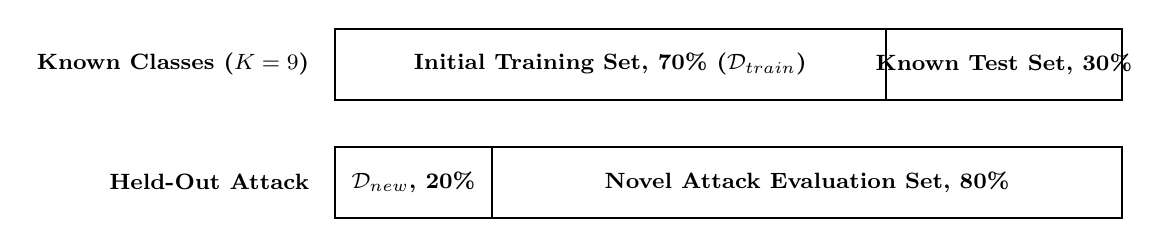
\begin{tikzpicture}
    % known classes
    \draw[line width=0.75pt] (0,1.5) rectangle (7,2.4);
    \draw[line width=0.75pt] (7,1.5) rectangle (10,2.4);
    \node at (3.5,1.95) {\bf\footnotesize Initial Training Set, 70\% ($\mathcal{D}_{\text{train}}$)};
    \node at (8.5,1.95) {\bf\footnotesize Known Test Set, 30\%};
    \node[left] at (-0.2,1.95) {\bf\footnotesize Known Classes ($K = 9$)};
    % held-out attack
    \draw[line width=0.75pt] (0,0) rectangle (2,0.9);
    \draw[line width=0.75pt] (2,0) rectangle (10,0.9);
    \node at (1,0.45) {\bf\footnotesize $\mathcal{D}_{\text{new}}$, 20\%};
    \node at (6,0.45) {\bf\footnotesize Novel Attack Evaluation Set, 80\%};
    \node[left] at (-0.2,0.45) {\bf\footnotesize Held-Out Attack};
  \end{tikzpicture}
  \caption{Leave-One-Attack-Out data partitioning strategy showing training, adaptation, and evaluation splits}
  \label{fig:loao_split}
\end{figure}

\begin{table}[!ht]
\centering
\small
\setlength{\tabcolsep}{5pt}
\renewcommand{\arraystretch}{1.2}
\caption{Adaptation and evaluation dataset splits across the four held-out attack scenarios}
\label{tab:loao_splits_pw}
\begin{tabular}{|l|l|r|r|r|}
\hline
\textbf{Held-Out Attack} & \textbf{Volumetric Regime} & \textbf{Adaptation Batch ($M$)} & \textbf{Evaluation Batch} & \textbf{Dynamic Buffer ($|\mathcal{B}|$)} \\ \hline
MITM       & Low Volume    & 207      & 832      & 900 flows ($k = 100$) \\
Ransomware & Medium Volume & 2{,}853  & 11{,}413 & 2{,}853 flows ($k = 317$) \\
XSS        & High Volume   & 2{,}903  & 11{,}616 & 2{,}898 flows ($k = 322$) \\
Backdoor   & High Volume   & 3{,}742  & 14{,}968 & 3{,}735 flows ($k = 415$) \\ \hline
\end{tabular}
\end{table}

\subsection{Implementation Platform}
\label{subsec:platform}

The entire framework was implemented in Python 3.9 using standard scientific computing and machine learning libraries. All experiments were executed on general-purpose CPU cores without GPU acceleration, reflecting realistic edge gateway hardware. Table~\ref{tab:platform} details the experimental execution environment, and Table~\ref{tab:hyperparameters} summarizes the operational module hyperparameters.

\begin{table}[htpb]
\centering
\small
\renewcommand{\arraystretch}{1.3}
\caption{Hardware and software experimental environment}
\label{tab:platform}
\begin{tabular}{|p{4.2cm}|p{8.5cm}|}
\hline
\textbf{Component} & \textbf{Specification / Library Version} \\ \hline
Processor Architecture & ARM-based Multi-Core Processor (CPU-only execution) \\
Host Memory (RAM)      & 16 GB unified memory \\
Operating System       & macOS Darwin 24.3.0 \\
Programming Language   & Python 3.9.6 (64-bit) \\
Machine Learning       & scikit-learn 1.6.1 (\texttt{RandomForestClassifier}, \texttt{IsolationForest}) \\
Data Manipulation      & pandas 2.3.3, NumPy 2.0.2 \\
Visualization          & Matplotlib 3.10.0, Seaborn 0.13.2 \\
Reproducibility        & Global pseudorandom seed: 42 \\ \hline
\end{tabular}
\end{table}

\begin{table}[htpb]
\centering
\small
\renewcommand{\arraystretch}{1.3}
\caption{Operational hyperparameters and module configuration settings}
\label{tab:hyperparameters}
\begin{tabular}{|p{4.5cm}|p{8.2cm}|}
\hline
\textbf{Module} & \textbf{Parameter Configuration} \\ \hline
M2 Random Forest Classifier & $B = 100$ trees, maximum depth $d_{\max} = 20$, Gini criterion \\
M3 Isolation Forest Screener & $T = 100$ trees, subsample size $\psi = 256$, contamination = auto \\
Static Replay Baseline     & Fixed quotas: $k \in \{25, 50, 100, 200, 500\}$ flows per class \\
M5 Dynamic Replay Manager  & Floor $k_{\min} = 100$, Total ceiling $N_{\text{cap}} = 5{,}000$ ($k_{\max} = 555$) \\
Data Partitioning Ratio    & Known classes: 70/30; Held-out zero-day attack: 20/80 \\ \hline
\end{tabular}
\end{table}

To ensure complete experimental reproducibility, a fixed global pseudorandom seed of 42 was maintained across all data partitioning splits, bootstrap resamples, tree feature subspace selections, and dynamic buffer draws.

\section{Summary}
\label{sec:summary_proposed_work}

This chapter presented the theoretical formulation, architectural design, and operational execution of the proposed two-stage continual intrusion detection framework for IoT edge gateways. We analyzed the fundamental limitations of static closed-world classifiers, established seven core functional and non-functional requirements, and detailed the seven operational modules of the system. 

Through mathematical analysis of decision tree induction and Gini impurity reduction under class imbalance, we demonstrated why static replay buffers inevitably induce severe catastrophic forgetting when novel attacks exhibit large volumetric surges. To overcome this limitation, we introduced the volume-aware Dynamic Replay rule, which scales the historical exemplar buffer proportionally with incoming attack volume while enforcing strict hardware memory bounds ($< 1$~MB) and sub-0.1~second retraining latency. Finally, we defined the TON\_IoT telemetry benchmark, the feature de-identification protocol, and the leave-one-attack-out evaluation methodology. Chapter~\ref{chap:results_and_discussion} presents the extensive empirical results and comparative analysis across all evaluation scenarios.
